\chapter{The Proposed Approach to the Problem}
\begin{itemize}
    \item For this project, we would like to compare different methods in this multi-robot task. In the comparation, we would like to compute the average time consumption for each model. According to the paper by Kohene\cite{Kohonen1998}, the computational complexity is $O(S2)$, where S is the size of the sample. Thus, we would like to investigate the computational complexity for these models. 
    
    \item We also want to re-produce the two SOM methods (K output neurons and KM output neurons) proposed by Anmin. 
    \begin{itemize}
        \item For small scale problems (K $<$ 8 and $M < 8$), we are going to compare the SOM results with the brute force method in terms of accuracy ( student-t test) and variance ( chi-square test)
        \item For large scale problems ( K or M $>$ 8), we are going to compare the time complexicity between the SOM methods vs. the brute force method
    \end{itemize}
    and compare the SOM result with brute force method's result for small scale problem, in terms of
    
    \item Moreover, we are still thinking about improving the SOM algorithm based genetic algrithms. After the improvement, we would like to compare the running time for these algorithms. 
    \item As shown in Figure \ref{fig-3}}, we have found that most of the time, the SOM is providing us very promising result comparing to the brute force result (Total traveling path 9.25 vs. 9.23);   While sometimes, the SOM will lead to vibration of robots between targets (as shown in Figure \ref{fig-4}). This vibration will lead to the SOM solution worse than the brute force solution (31.56 vs. 19.65)
    \begin{figure}[h]
  \centering
  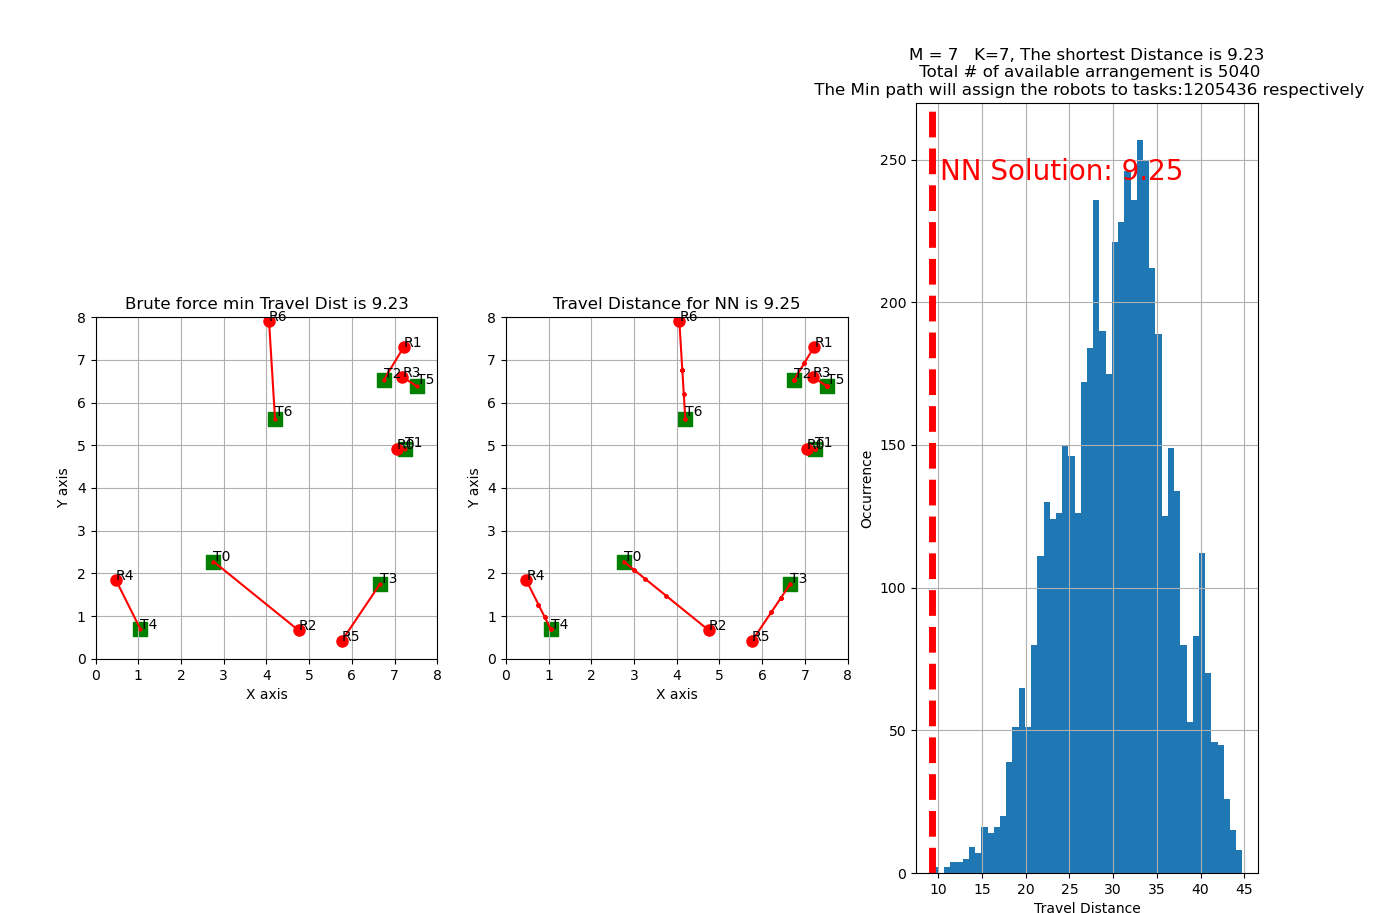
\includegraphics[width=15cm]{Pictures/Anmin Repeat1.png}
  \caption{The SOM is providing result very close to brute force result in most of the case with K = 7, M = 7, on a 8 by 8 Grid}
  \label{fig-3}
\end{figure}

\begin{figure}[h]
  \centering
  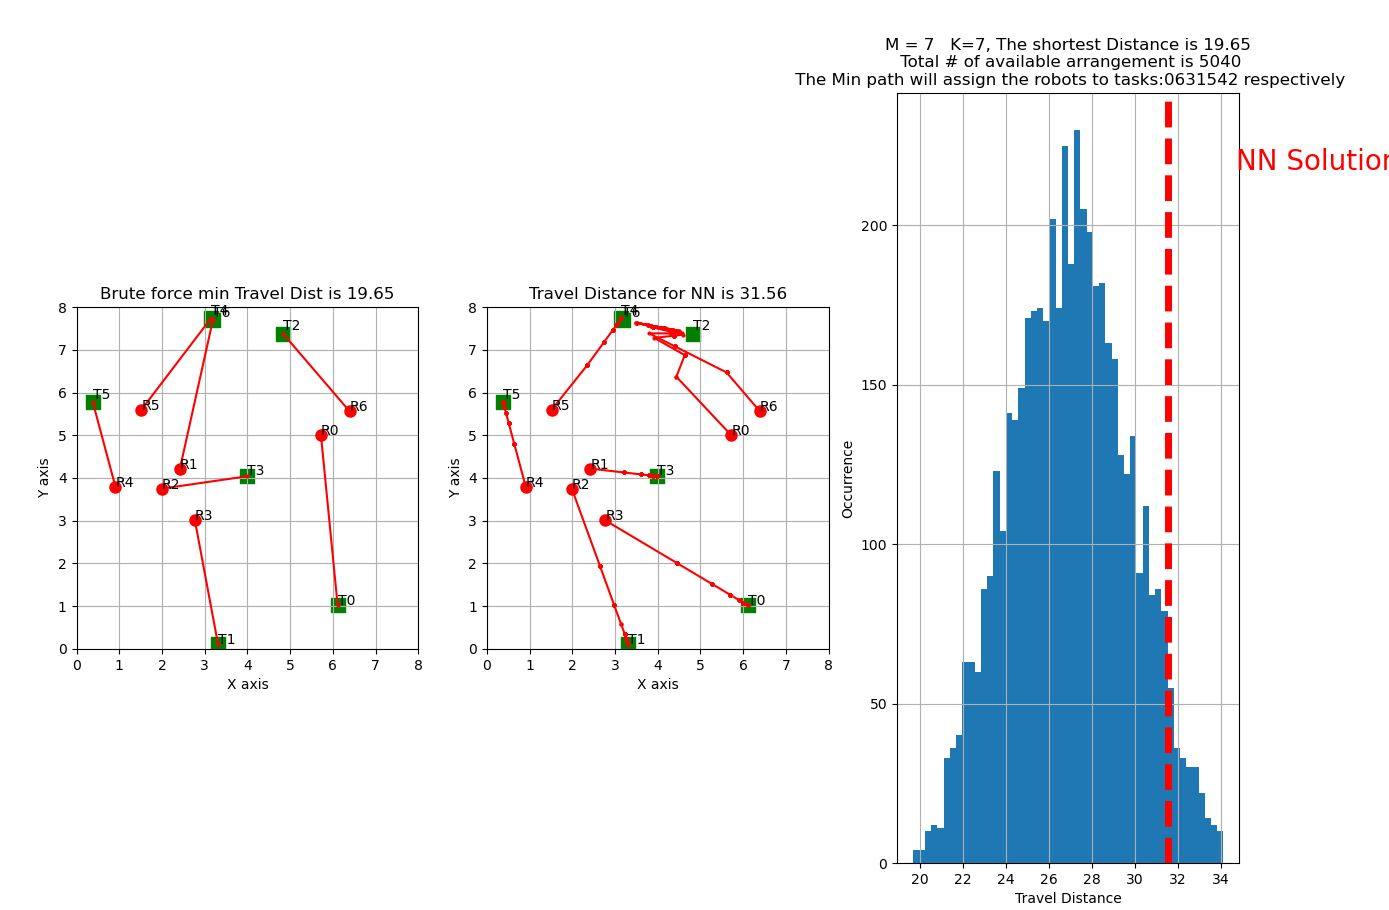
\includegraphics[width=15cm]{Pictures/Anmin-Notgood.JPG}
  \caption{The SOM sometimes vibrate and then provide a bad result comparing to brute force result with K = 7, M = 7, on a 8 by 8 Grid}
  \label{fig-4}
\end{figure}
\end{itemize}


